\subsection{Introducción}\label{header-n2}
Este caso, como ya se ha mencionado, es el resultado de las pruebas
realizadas con anterioridad, tanto en el laboratorio como con la
simulación de varios casos, donde se fueron implementando utilidades y
funciones de ejemplos de OpenFOAM. A continuación se presenta la
estructura del caso:

\dirtree{%
 .1 $<$case$>$.
 .2 0.
 .3 alpha.water.
 .3 alpha.water.orig.
 .3 epsilon.
 .3 k.
 .3 nut.
 .3 nuTilda.
 .3 p\_rgh.
 .3 U.
 .2 constant.
 .3 g.
 .3 transporProperties.
 .3 turbulenceProperties.
 .2 system.
 .3 blockMeshDict.
 .3 topoSetDict1.
 .3 topoSetDict2.
 .3 topoSetDict3.
 .3 setFields.
 .3 fvSchemes.
 .3 fvSolution.
 .3 controlDict.
 .3 singleGraph.
 .3 probes.
}

\subsection{Definición del caso}\label{header-n9}

\begin{figure}
\centering
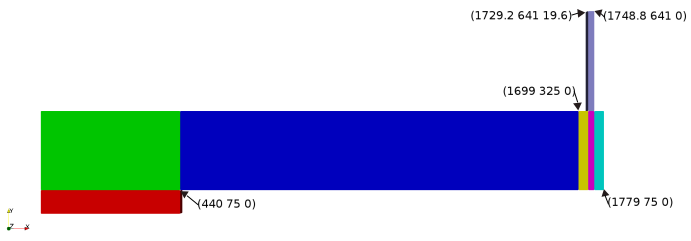
\includegraphics[width=\linewidth]{DimCanal2D.png}
\caption{Imagen con la representación de las medidas mínimas necesarias}
\label{fig:DimCanal2D}
\end{figure}

\begin{figure}
\centering
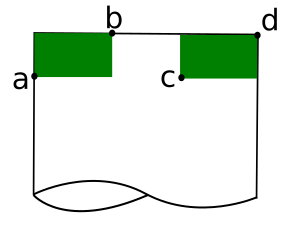
\includegraphics[width=0.3\linewidth]{diafCanal2D.png}
\caption[Representación del diafragma]{Representación del diafragma, colocado en la parte superior del tubo de salida}
\label{fig:diafCanal2D}
\end{figure}

\begin{figure}
\centering
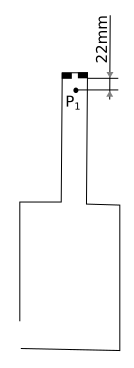
\includegraphics[width=0.2\linewidth]{probeCanal2D.png}
\caption{Boceto que representa el punto de medición de la presión}
\label{fig:probeCanal2D}
\end{figure}

\begin{itemize}
\item
  Objetivos planteados:

  \begin{itemize}
  \item
    Llenar el canal hasta sobrepasar la altura de la entrada de agua a
    la cámara. Esto hará que la caida de agua y entrada en la cámara no
    sea tan brusca y se pueda medir adecuadamente la presión a la
    salida.
  \item
    Obtener la altura media del volumen de agua, dentro de la cámara.
  \item
    Hallar el flujo de salida a través del diafragma.
  \item
    Calcular el valor de la presión manométrica aguas arriba del
    diafragma.
  \end{itemize}
\item
  Definición del modelo con \emph{blockMeshDict}

  \begin{itemize}
  \item
    En este caso la malla definida, es estructurada y hexaédrica,
    compuesta por 7 bloques y una anchura de celda de aproximadamente
    \(2 mm\).
  \item
    Se definen los siguientes contornos: \emph{leftWall, rightWall,
    lowerWall, atmosphere, aoutflow, topWall, defaultFaces}.
  \item
    Las dimensiones expresadas por las posiciones de los vértices se
    multiplican por 0,001 para convertirlas a metros, el orden también
    es importante \cite{guideblockMesh}. En la imagen \autoref{fig:DimCanal2D} se definen las
    medidas consideradas para este caso.

  \end{itemize}
\item
  Propiedades físicas:

  \begin{itemize}
  \item
    Las propiedades del agua se mantienen como en el caso
    \emph{``damBreak''} donde la \emph{viscosidad cinemática \texttt{nu}}
    se definía como \(1\times10^{-6} m^2/s\) y la \emph{densidad
    (\texttt{rho})} de \(1000 kg/m^3\).
  \item
    En cambio para el aire se establece una
    \(\nu=1,5 \times ^{-5} m^2/s\) y una \(\rho=1.2kg/m^3\).
  \end{itemize}
\item
  Condiciones iniciales:

  \begin{itemize}
  \item
    Se comprueba que los contornos definidos en \emph{blockMeshDict}
    correspondan con los definidos para cada variable principal
    implicada en el caso.
  \item
    Para no tener que complicar el modelo en exceso, se incluye la
    utilidad TopoSet \cite{toposet},
    que permitirá añadir la pared que delimitará la cámara (con una
    abertura de \(25mm\) en \emph{y} para dejar pasar el agua) y el
    diafragma (representado por una rendija rectangular de \(19,6mm\), en
    \emph{x}) en la parte superior de la chimenea, en \autoref{fig:diafCanal2D} se puede ver la representación de los puntos para el diafragma que acontinuación se definen.

    Por tanto, se generan tres diccionarios, ubicados en
    \lstinline[style=bash]{./system/}, de forma que las celdas
    comprendidas en los prismas definidos (como en el diccionario
    \emph{setFieldsDict}) se conviertan en paredes (medidas expresadas
    en metros):

    \begin{itemize}
    \item
      Pared vertical: \lstinline[style=bash]{(1.693 0.1 0) (1.699 0.325 1)}.
    \item
      Pared diafragma izquierda: \lstinline[style=c++]{a=(1.7292 0.639 0);b=(1.73275 0.641 1)}.
    \item
      Pared diafragma derecha: \lstinline[style=c++]{c=(1.74525 0.639 0);d=(1.7488 0.641 1)}.



    \end{itemize}
  \item
    La condición inicial del volumen de agua se define mediante dos
    prismas, uno hasta la compuerta (a \(600mm\) en $x$ y
    \(220mm\) en $y$); y el otro sobrepasando la entrada de agua
    a la cámara (hasta una altura en el canal de \(45mm\)), expresado en
    el diccionario \emph{setFieldsDict} (en metros):

    \begin{itemize}
    \item
      Volumen1= \lstinline[style=bash]{(0 0 -1) (.60 .22 1)}.
    \item
      Volumen2= \lstinline[style=bash]{(.60 0 -1) (1.779 .12 1)}.
    \end{itemize}
  \end{itemize}
\item
  Obtención de resultados:

  \begin{itemize}
  \item
    Las funciones introducidas en
    \lstinline[style=bash]{./system/controlDict} servirán para hallar
    un fichero con los valores de la presión en un punto a lo largo del
    tiempo; así como, el flujo a través del diafragma.

    \begin{itemize}
    \item
      El punto para medir la presión se obtiene del ensayo, más adelante
      se detallará. Por otro lado, el centroide más aproximado que
      corresponda a la ubicación se puede hallar con la función
      \texttt{singleGraph}, donde se estima un punto de inicio y otro
      final para hallar los valores en los centroides intermedios (se
      guardan en directorios separados por el paso del tiempo). En este
      caso, representado en \autoref{fig:probeCanal2D}, el punto definido en el diccionario
      \lstinline[style=bash]{./system/probes}, expresado en metros, es:
      \lstinline[style=bash]{(1.739 0.618 0.0098)}.



    \item
      La función para hallar el flujo de salida (\emph{outletFlux}) se
      determina en el propio \emph{controlDict}, donde se define el
      campo a calcular
      \texttt{rhoPhi}(\(\frac {kg}{m^3} \frac {m}{s}= \frac {kg}{s} \cdot \frac {1}{m^2}\))
      y sobre qué región \texttt{outflow}. Estos resultados se guardarán
      a lo largo del tiempo en un solo fichero.
    \end{itemize}
  \item
    La altura del agua dentro de la cámara se determina una vez simulado
    el caso, a partir de un \emph{script} generado en lenguaje de
    \emph{Python} y ejecutado desde ParaView. Este \emph{script},
    completamente explicado en \emph{ali-ramezani/OpenFOAM-Tips}\footnote{\url{https://github.com/ali-ramezani/OpenFOAM-Tips}},
    se genera desde la opción \lstinline[style=bash]{Tools/Start Trace} del menú de
    ParaView; realizando los pasos de acontinuación; y volviendo al
    menú, a \lstinline[style=bash]{Tools/Stop Trace}.

    \begin{itemize}
    \item
      Abrir desde \emph{ParaView} el fichero \emph{a.foam} del caso
      (fichero vacio que sirve para post-procesar los resultados de las
      carpetas de cada paso del tiempo desde ParaView. Al ejecutar
      \texttt{paraFoam} este fichero se genera automáticamente para
      mostrar los resultados; en cambio, si se abre \emph{ParaView} se
      tendrá que crear a parte).
    \item
      Trasladar la información a los puntos usando el filtro
      \emph{CellDataPointData}.
    \item
      Se realiza un corte en el plano $y$ en la posición
      \lstinline[style=bash]{[1.699, 0.3, 0.05]} donde comienza la cámara.
    \item
      Crear un contorno para \lstinline[style=bash]{alpha.water=0.5}, donde se encuentra
      la interfase.
    \item
      Añadir un nuevo escalar que almacene los datos del nivel del agua.
    \item
      Integrar el contorno de la superficie 3D para obtener un valor
      promedio del nivel del agua.
    \end{itemize}

    Se dejan los campos mínimos necesarios para obtener la altura de la
    SLL, ya que no se requiere la visualización gráfica. Finalmente, se
    añaden al \emph{script} las ordenes convenientes para guardar en un
    fichero CSV el resultado de la división \emph{ylevel/Area} a lo
    largo del tiempo.
  \end{itemize}
\end{itemize}

\subsection{Ejecución}\label{header-n140}

El procesado se puede realizar ejecutando el \emph{script}
\texttt{Allrun} donde se describen las siguientes instrucciones:

\begin{figure}[hb]
\centering
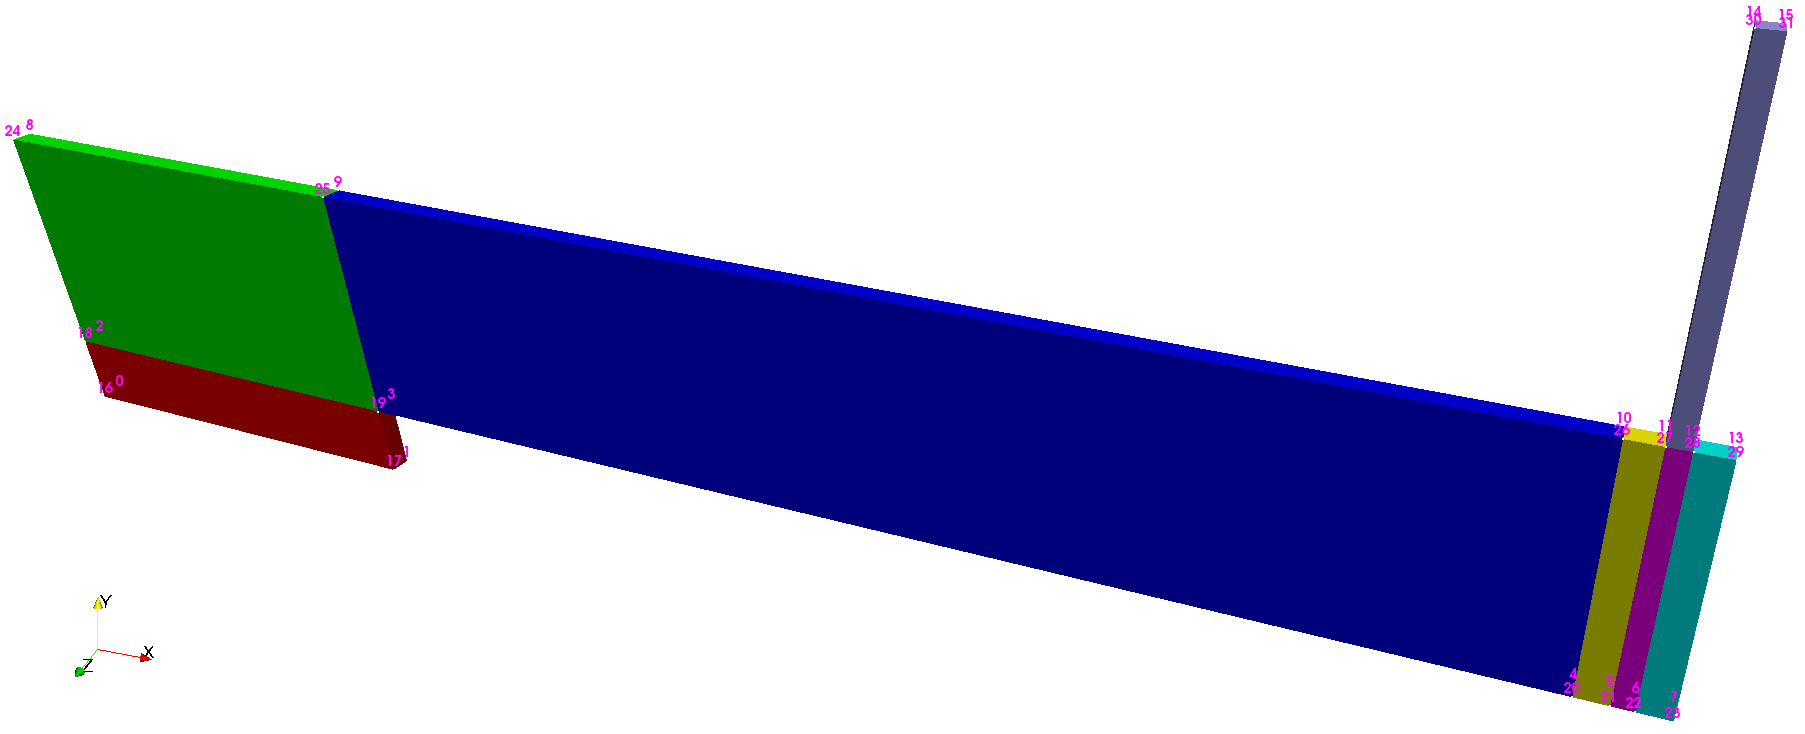
\includegraphics[width=0.8\linewidth]{blockcanal2D19.png}
\caption{Representación de los vértices y bloques del modelo}
\label{fig:blockcanal2D19}
\end{figure}

\begin{figure}[hb]
\centering
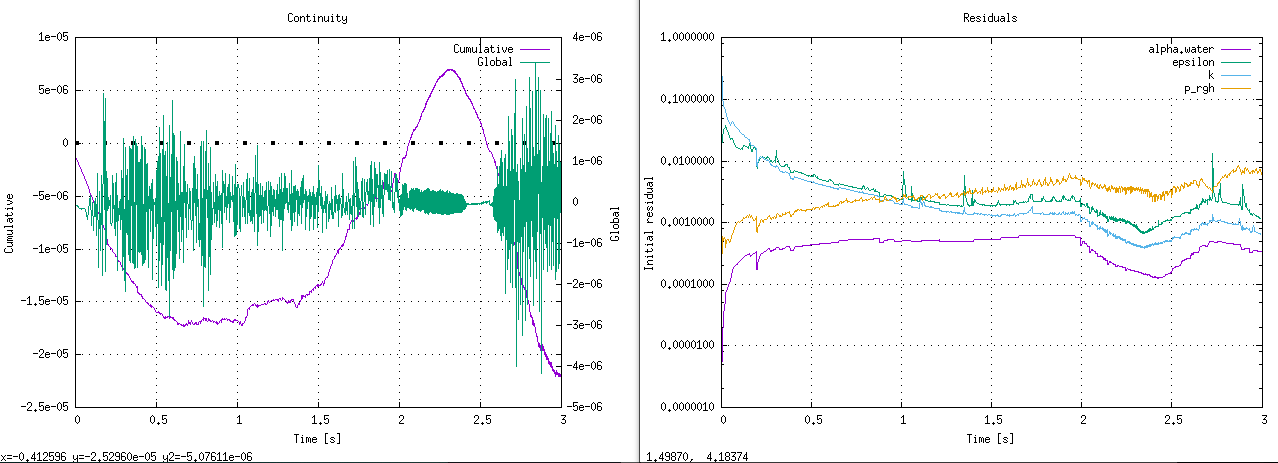
\includegraphics[width=\linewidth]{residualsCanal2D19.png}
\caption{Residuos del caso ejecutado}
\label{fig:residualsCanal2D19}
\end{figure}

\begin{enumerate}
\def\labelenumi{\arabic{enumi}.}
\item
  Mediante la orden \texttt{blockMesh}, se descompone el dominio en sus
  tres ejes por hexaedros y se escriben los datos de los puntos, caras,
  celdas de la malla. La representación de los vértices se puede apreciar en \autoref{fig:blockcanal2D19}.

\item
  La adición de las diferentes paredes se implementa como en el ejemplo
  de
  \lstinline[style=bash]{\$FOAM\_run/multiphase/interFoam/les/nozzleFlow2D}:

\begin{lstlisting}[style=c++]
for i in 1 2 3
do
    runApplication -s $i \
        topoSet -dict system/topoSetDict${i}

    runApplication -s $i \
        subsetMesh -overwrite c0 -patch internalWalls
done
\end{lstlisting}

\item
  La condición inicial del agua se agrega mediante la orden:
  \texttt{setFields}
\item
  Finalmente, se ejecuta \texttt{interFoam\ \&}, y se visualiza el caso desde \emph{ParaView} para ver el movimiento del agua en el canal a lo largo del tiempo, ver imagen \autoref{fig:canal2D19}. Esta orden se ejecuta en segundo plano para
  lanzar, al mismo tiempo, la orden
  \texttt{pyFoamPlotWatcher.py\ log.interFoam}, la cual obtiene del
  registro los residuos de las variables principales, representados en la gráfica \autoref{fig:residualsCanal2D19}.

\end{enumerate}

\begin{figure}
\centering
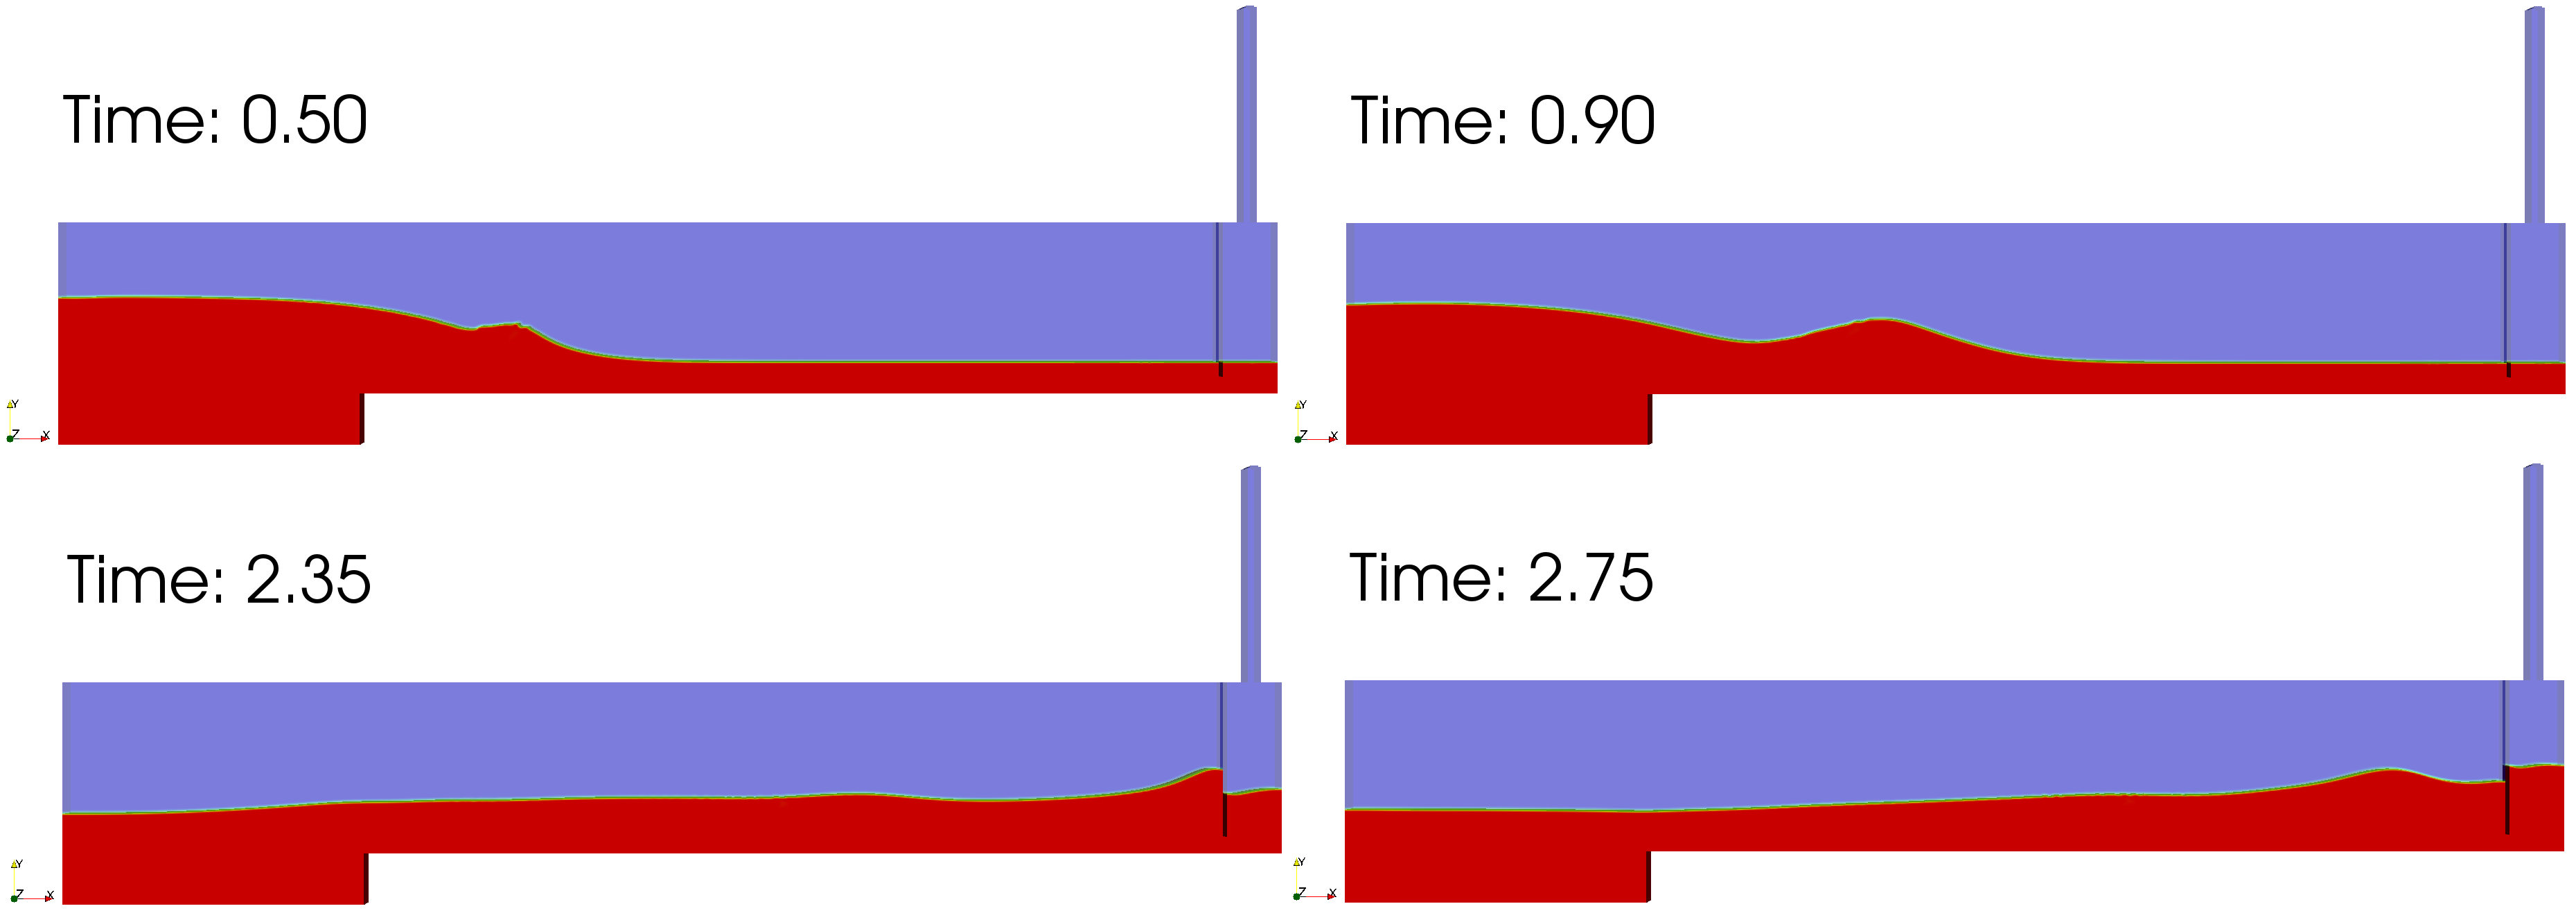
\includegraphics[width=\linewidth]{canal2D19.png}
\caption{Imágenes de la visualización del caso desde ParaView}
\label{fig:canal2D19}
\end{figure}

\subsection{Resultados}\label{header-n173}

Una vez ejecutado el caso se pueden obtener los siguientes resultados:

\begin{figure}
\centering
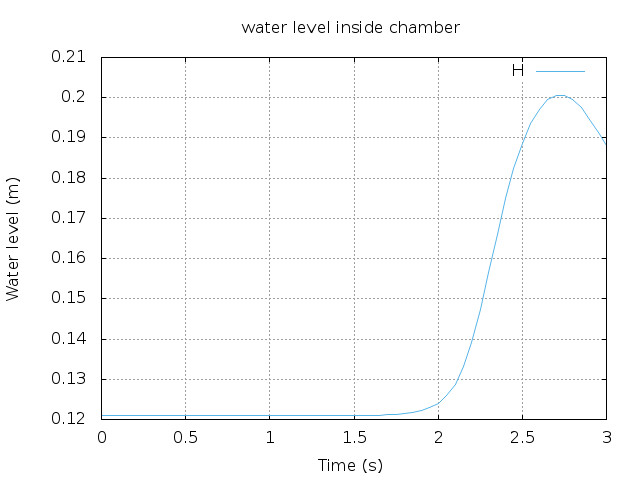
\includegraphics[width=0.8\linewidth]{WLCanal2D19.jpg}
\caption[Gráfica del nivel del agua]{Gráfica del nivel del agua dentro de la cámara a lo largo del tiempo}
\label{fig:WLCanal2D19}
\end{figure}

\begin{figure}
\centering
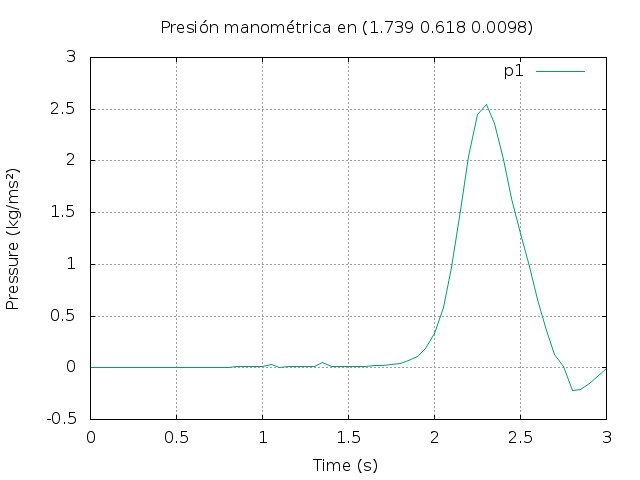
\includegraphics[width=0.8\linewidth]{PmCanal2D19.jpg}
\caption{Medida de la Presión manométrica a lo largo del tiempo}
\label{fig:PmCanal2D19}
\end{figure}

\begin{enumerate}
\def\labelenumi{\arabic{enumi}.}
\item
  Del fichero \textless{}./log.blockMesh\textgreater{} se puede hallar la siguiente información del modelo:

  \begin{itemize}
  \item
    \textbf{Número de celdas}: 121.190
  \item
    \textbf{Dominio (\emph{boundingBox})}: (0 0 0) (1.779 0.641
    0.0196) m.
  \end{itemize}
\item
  Para ejecutar el script de \emph{Python} y hallar la \textbf{altura del nivel
  de agua en la cámara}:

  \begin{itemize}
  \item
    Completar de forma adecuada los datos de entrada, al comienzo del
    \emph{script}.
  \item
    Ejecutar el \emph{script} desde ParaView en
    \lstinline[style=bash]{Herramientas/Python Shell/Ejecutar script}.
  \end{itemize}

  El archivo de salida se guarda en la carpeta del caso, listo para
  trazar el gráfico desde una herramienta indicada para ello. En este
  caso se utiliza un \emph{script} \lstinline[style=bash]{./RunWL} para
  generarlo automáticamente desde Gnuplot, obteniendo el resultado de la altura del agua en la cámara respecto del tiempo mostrado en \autoref{fig:WLCanal2D19}.

\item
  La \textbf{presión manométrica} en el punto mencionado, se escribe en el
  fichero \lstinline[style=bash]{./portProcessing/probes/0/p}. No
  obstante, el valor de ésta es negativo, con lo que se utiliza un
  \emph{script} generado en \emph{ParaView} para hallar esta medida.

  De forma análoga al proceso de obtención del nivel de agua dentro de
  la cámara, se lleva a cabo desde ParaView, a través de las instrucciones guardadas en el
  \emph{script} \lstinline[style=bash]{./prgh.py} que se ejecutará desde la consola de \emph{Python}, para escribir la solución de la presión en el tiempo, se realizan los siguientes pasos:  

  \begin{itemize}
  \item
    Desde el menú de \emph{ParaView} \lstinline[style=bash]{Tools/Start Trace}.

    \begin{itemize}
    \item
      Abrir el fichero \emph{a.foam}.
    \item
      Trasladar la información a los puntos con el filtro
      \emph{cellDataToPointData}.
    \item
      Crear un punto de muestreo \emph{probeLocation} en \lstinline[style=bash]{1.739, 0.618, 0.0098}.
    \item
      Aplicar el filtro \emph{Calculator} a la variable \emph{p\_rgh}.
    \end{itemize}
  \item
    Volver al menú y seleccionar \lstinline[style=bash]{Tools/Stop Trace}, para guardar
    estos pasos en el \emph{script}.
  \end{itemize}

  Para guardar los resultados a lo largo del tiempo se modifica la parte
  final del \emph{script} teniendo como referencia el anterior y
  resolviendo los errores con las respuestas halladas en foros de internet. Este archivo de datos se procesa desde Octave para dar la solución ofrecida en la imagen \autoref{fig:PmCanal2D19}.

\item
  Los resultados del \textbf{caudal a través del diafragma} se escriben durante
  la simulación en
  \lstinline[style=bash]{./postProcessing/outletFlux/0/surfaceRegion.dat},
  para gráficarlos se puede ejecutar el \emph{script}
  \lstinline[style=bash]{./RunPlotFlow}. 
  Dando como resultado la gráfica \autoref{fig:FlowRCanal2D19} del caudal respecto del tiempo.
\end{enumerate}

\begin{figure}
\centering
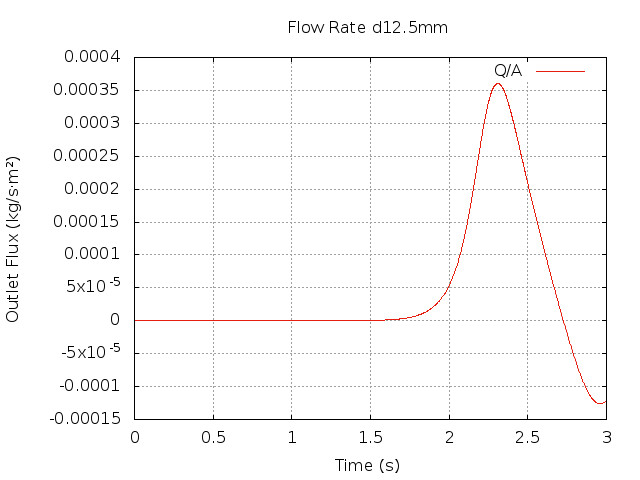
\includegraphics[width=0.8\linewidth]{FlowRCanal2D19.jpg}
\caption{Medida del caudal a través del diafragma}
\label{fig:FlowRCanal2D19}
\end{figure}

\subsection{Conclusiones}\label{header-n245}

Los valores del caudal y presión manométrica obtenidos, resultan muy
bajos, con lo que se realiza una segunda prueba, variando la anchura del
modelo de \(19,6 mm\) a \(80 mm\). Logrando un aumento del caudal y una
disminución en la presión manométrica, como se puede apreciar en la
gráfica de la imagen \autoref{fig:RmFrCanal2D80}.

\begin{figure}
\centering
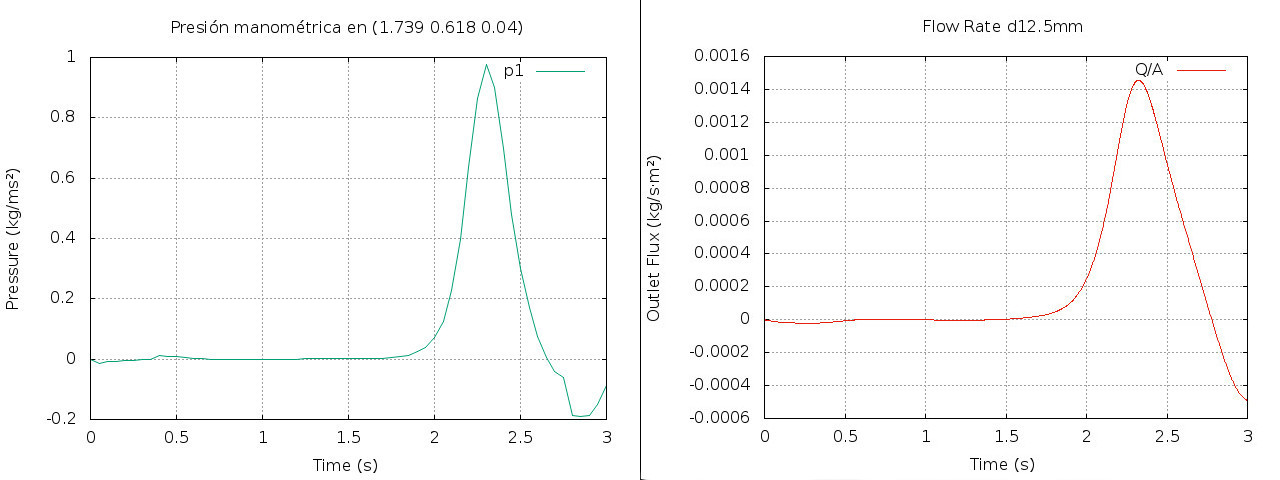
\includegraphics[width=\linewidth]{RmFrCanal2D80.jpg}
\caption[Presión manométrica y flujo de aire]{Presión manométrica aguas arriba del diafragma y flujo de aire a través del mismo}
\label{fig:RmFrCanal2D80}
\end{figure}

Aunque sea un caso en 2-D, OpenFOAM siempre opera en 3-D, las
variaciones del volumen de agua al modificar la anchura del modelo
resultan significativas para la solución. Junto con esto, también, se
han realizado diversas simplificaciones en el modelo (p.e. las
superficies curvas son convertidas a rectangulares), por ello los
resultados no resultan muy convincentes. En vez de tratar de adaptar
estos valores, se concluye que será necesario realizar el modelo en 3-D,
para que la solución, a la hora de compararla con la obtenida en el
ensayo, no difiera en exceso.
